%%% BAC solution 01 %%%
\documentclass{article}
\usepackage[margin=1in]{geometry}
\usepackage{amsmath, amssymb, amsfonts, enumitem, fancyhdr, pgfplots, tikz}
% need to set pgfplots compatibility (choose newest)
\pgfplotsset{compat=newest}
% get rid of paragraph indent
\setlength{\parindent}{0 pt}
% allow section.equation numbering
\numberwithin{equation}{section}
% allows you to copy-paste code segments. requires pygments, which can be
% installed from PyPI with pip install Pygments.
% warning: minted does NOT work with Texmaker if you have TeX Live installed
% on WSL but Texmaker installed natively on Windows!
%\usepackage{minted}
% alternative to minted that does not require Python, LaTeX only. listings is
% however disgusting out of the box and some setup is required.
\usepackage{listings, xcolor}
% makes clickable links to sections
\usepackage{hyperref}
% make the link colors blue, as well as cite colors. urls are magenta
\hypersetup{
    colorlinks, linkcolor = blue, citecolor = blue, urlcolor = magenta
}
% fancy pagestyle so we can use fancyhdr for fancy headers/footers
\pagestyle{fancy}
% add logo in right of header. note that you will have to adjust logo path!
\fancyhead[R]{
\includegraphics[scale = 0.15]{../bac_logo1.png}}
% don't show anything in the left and center header
\fancyhead[L, C]{}
% give enough space for logo by reducing top margin height, head separator,
% increasing headerheight. see Figure 1 in the fancyhdr documentation. if
% \topmargin + \headheight + \headsep = 0, original text margins unchanged.
\setlength{\topmargin}{-60 pt}
\setlength{\headheight}{50 pt}
\setlength{\headsep}{10 pt}
% remove decorative line in the fancy header
\renewcommand{\headrulewidth}{0 pt}

% color definitions for listings syntax highlighting. uses colors borrowed
% from the VS Code Dark+ and Abyss standard themes.
\definecolor{KwColor}{RGB}{153, 102, 184}     % keyword color
\definecolor{VarColor}{RGB}{86, 156, 214}     % variables/identifier color
\definecolor{StrColor}{RGB}{209, 105, 105}    % string color
\definecolor{CmtColor}{RGB}{106, 153, 85}     % comment color

% general listings configuration for all languages
\lstset{
    % change keyword, identifier, comment, string colors
    keywordstyle = \color{KwColor},
    commentstyle = \color{CmtColor},
    identifierstyle = \color{VarColor},
    stringstyle = \color{StrColor},
    % no spaces in strings
    showstringspaces = false,
    % monospace font by default
    basicstyle = \ttfamily,
    % tabsize 8 by default, this is not the 1960s
    tabsize = 4,
    % add line numbers to the left with gray typewriter font
    numbers = left,
    numberstyle = \color{gray}\ttfamily,
    % change distance from code block from 10 pt to 5 pt
    numbersep = 5 pt
}

% colors to use for Figure 1 in section 1.4. these are the RGB values returned
% by the matplotlib viridis colormap, produced using the following Python code:
%
% import matplotlib.cm as cm
% cm.viridis([0.1, 0.5, 0.9])
%
% a numpy.ndarray shape (3, 4) is returned, each row the RGBA values.
\definecolor{viridis_ichi}{rgb}{0.282623, 0.140926, 0.457517}
\definecolor{viridis_ni}{rgb}{0.127568, 0.566949, 0.550556}
\definecolor{viridis_san}{rgb}{0.741388, 0.873449, 0.149561}

% title, author, date
\title{Solution 1}
\author{Derek Huang\thanks{NYU Stern 2021, BAC Advanced Team.}}
\date{May 20, 2021}

\begin{document}

\maketitle
% need to include this after making title to undo the automatic
% \thispagestyle{plain} command that is issued.
\thispagestyle{fancy}

\section{Set theory}

\subsection{Partition of $ \mathbb{R} $}

\textit{Solution 1.} Consider the infinite sequence
$ \left\{1 - \frac{1}{k}\right\}_{k \in \mathbb{N}} $. Note that
$ \lim_{k \rightarrow \infty}\left(1 - \frac{1}{k}\right) = 1 $ and that the
sequence is strictly monotone increasing, as
$ 0 < \frac{1}{2} < \frac{2}{3} < \ldots < 1 $. Now let us define $ A_k $,
$ \forall k \in \mathbb{N} $, such that
\begin{equation*}
    A_k \triangleq \left[1 - \frac{1}{k}, 1 - \frac{1}{k + 1}\right)
\end{equation*}

It's clear that $ A_1, A_2 \ldots $ are mutually disjoint and that
$ \bigcup_{k \in \mathbb{N}}A_k = \left[0, \frac{1}{2}\right) \cup
\left[\frac{1}{2}, \frac{2}{3}\right) \cup \ldots = [0, 1) $ . Therefore,
\begin{equation*}
    P = \bigcup_{k \in \mathbb{N}}\{A_k\}
\end{equation*}

\medskip

\textit{Solution 2.} Consider the infinite geometric series
$ \sum_{k = 0}^\infty r^k $, where $ r \in (0, 1) $. Since $ |r| < 1 $, we
know that $ \sum_{k = 0}^\infty r^k $ converges. In particular, by the
formula for the convergent geometric series, we see that
\begin{equation*}
    (1 - r)\sum_{k = 0}^\infty r^k = (1 - r)\frac{1}{1 - r} = 1
\end{equation*}

Let $ S_{k; r} \triangleq (1 - r)\sum_{j = 0}^kr^j $,
$ \forall k \in \mathbb{N} \cup\{0\} $. Since the terms of
$ \{S_{k; r}\}_{k \in \mathbb{N}} $ are strictly monotone increasing, as
$ 1 - r < (1 - r)(1 + r) < (1 - r)(1 + r + r^2) < \ldots $, let us define
$ A_{k; r} $, $ \forall k \in \mathbb{N} \cup \{0\} $, such that
\begin{equation*}
    A_{k; r} \triangleq [S_{k; r}, S_{k + 1; r})
\end{equation*}

It's clear that $ A_{0; r}, A_{1; r}, \ldots $ are mutually disjoint and that
$ [0, 1 - r) \cup \bigcup_{k \in \mathbb{N} \cup\{0\}}A_{k; r} = [0, 1) $.
Therefore,
\begin{equation*}
    P_r \triangleq \{[0, 1 - r)\} \cup
    \bigcup_{k \in \mathbb{N}\cup\{0\}}\{A_{k; r}\}
\end{equation*}

$ \forall r \in (0, 1) $, $ P_r $ is a partition of $ [0, 1) $ into an
infinite number of half-open intervals.

\subsection{Slicing the unit circle}

\textit{Solution.} Note that $ \tilde{U} \triangleq \{\mathbf{x} \in U :
x_1 \ne 0, x_2 \ne 0\} $, as no point in $ \tilde{U} $ lies on the $ x_1 $ or
$ x_2 $ axes. Noting that $ A \subset U $, we see that $ A = U \setminus
\tilde{U} $, and can therefore write $ A \triangleq
\{\mathbf{x} \in U : x_1 = 0\} \cup \{\mathbf{x} \in U : x_2 = 0\} $.

\subsection{Countably infinite intersection}

\textit{Solution.} Note that $ -\lim_{k \rightarrow \infty}e^{-k} = 0 $ and
that $ 1 + \lim_{k \rightarrow \infty}e^{-k} = 1 $. However, note that
$ \forall k \in \mathbb{N} $, $ -e^{-k} < 0 $, $ 1 + e^{-k} > 1 $. Therefore,
$ \bigcap_{k \in \mathbb{N}}A_k = [0, 1] $. This result can be seen by
noting that $ [0, 1] $ is a subset of each open interval in
$ \{A_k\}_{k \in \mathbb{N}} $, where $ A_k \subset A_{k + 1} $,
$ \forall k \in \mathbb{N} $. The intervals therefore more and more tightly
wrap $ [0, 1] $, but since they do not contain their endpoints, in the limit
the left endpoint converges to $ 0 $ and the right endpoint to $ 1 $, which
are included since the endpoints never attain these values.

\subsection{$ \ell^p $ norm balls}

\textit{Solution.} Consider Figure \ref{fig:p_norm_balls}, which plots the
boundaries of $ \bar{B}_{2, \ell^1}(\mathbf{0}, 1) $,
$ \bar{B}_{2, \ell^2}(\mathbf{0}, 1) $, and
$ \bar{B}_{2, \ell^\infty}(\mathbf{0}, 1) $.

\begin{figure}[h!]
    \centering
    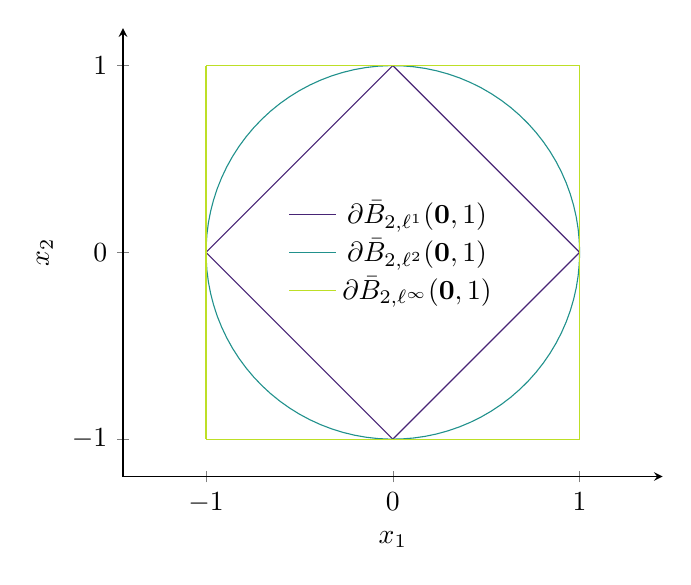
\begin{tikzpicture}
        \begin{axis}[
            % where to draw the axis lnes
	        axis lines = left,
	        xmin = -1.2, xmax = 1.2, ymin = -1.2, ymax = 1.2,
	        % make the axes equal length
	        axis equal,
	        xlabel = $ x_1 $,
	        ylabel = {$ x_2 $},
	        % set x and y ticks
	        xtick = {-1, 0, 1},
	        ytick = {-1, 0, 1},
	        % put legend in middle of plot, anchored to north, no border
	        legend style = {
	            at = {(0.5, 0.64)}, anchor = north, draw = none
	        }
	    ]
	        %% plotting the 1-norm ball %%
	        \addplot[
	            domain = 0:1,
	            color = viridis_ichi,
	            % don't track plot when creating legend
	            forget plot
	        ]{1 - x};
	        \addplot[
	            domain = 0:1,
	            color = viridis_ichi,
	            % don't track plot when creating legend
	            forget plot
	        ]{x - 1};
	        \addplot[
	            domain = -1:0,
	            color = viridis_ichi,
	            % don't track plot when creating legend
	            forget plot
	        ]{x + 1};
	        \addplot[
	            domain = -1:0,
	            color = viridis_ichi
	        ]{-1 - x};
	        \addlegendentry{$ \partial\bar{B}_{2, \ell^1}(\mathbf{0}, 1) $}
	        %% plotting the 2-norm ball %%
	        \addplot[
	            % note that the domain is in degrees
	            domain = 0:360,
	            % need more samples because we are plotting a curve
	            samples = 100,
	            color = viridis_ni
	        ]({cos(x)}, {sin(x)});
	        \addlegendentry{$ \partial\bar{B}_{2, \ell^2}(\mathbf{0}, 1) $}
	        %% plotting the max-norm ball %%
	        \addplot[
	            domain = -1:1,
	            color = viridis_san,
	            % don't track plot when creating legend
	            forget plot
	        ]({-1}, {x});
	        \addplot[
	            domain = -1:1,
	            color = viridis_san,
	            % don't track plot when creating legend
	            forget plot
	        ]({1}, {x});
	        \addplot[
	            domain = -1:1,
	            color = viridis_san,
	            % don't track plot when creating legend
	            forget plot
	        ]({x}, {-1});
	        \addplot[
	            domain = -1:1,
	            color = viridis_san
	        ]({x}, {1});
	        %\addlegendentry{$ \bar{B}_{2, \ell^\infty}(\mathbf{0}, 1) $}
	        \addlegendentry{$ \partial\bar{B}_{2, \ell^\infty}(\mathbf{0}, 1) $}
	    \end{axis}
    \end{tikzpicture}
    \caption{
        The boundaries of $ \bar{B}_{2, \ell^1}(\mathbf{0}, 1) $,
        $ \bar{B}_{2, \ell^2}(\mathbf{0}, 1) $, and
        $ \bar{B}_{2, \ell^\infty}(\mathbf{0}, 1) $.
    }
    \label{fig:p_norm_balls}
\end{figure}

It's clear that $ \bar{B}_{2, \ell^\infty}(\mathbf{0}, 1) $ contains both
$ \bar{B}_{2, \ell^1}(\mathbf{0}, 1) $ and
$ \bar{B}_{2, \ell^2}(\mathbf{0}, 1) $. In fact, it is true in general that
$ \forall n \in \mathbb{N} + 1 $, $ \forall \mathbf{x} \in \mathbb{R}^n $,
$ \forall r \in (0, \infty) $, that $ \bar{B}_{n, \ell^1}(\mathbf{x}, r)
\subset \bar{B}_{n, \ell^2}(\mathbf{x}, r) \subset
\bar{B}_{n, \ell^\infty}(\mathbf{x}, r) $, which agrees with intuition.

\subsection{Complex numbers}

\textit{Proof.} $ \forall r \in \mathbb{R} $, $ r = r + 0i \in \mathbb{C}
\Rightarrow \mathbb{R} \subseteq \mathbb{C} $. Since $ \forall c \in
\mathbb{R} \setminus \{0\} $, $ r + ci \notin \mathbb{R} $, then
$ \mathbb{R} \ne \mathbb{C} \Rightarrow \mathbb{R} \subset \mathbb{C} $.

\section{Probability}

\subsection{Event unions}

\textit{Proof.} Note that $ A \cup B = A \cup (B \setminus A) $, a disjoint
union. Furthermore, note that $ B = (B \setminus A) \cup (A \cap B) $, also a
disjoint union. By the 3\textsuperscript{rd} Kolmogorov axiom, we thus know
that $ \mathbb{P}(A \cup B) = \mathbb{P}(A) + \mathbb{P}(B \setminus A) $ and
that $ \mathbb{P}(B) = \mathbb{P}(B \setminus A) + \mathbb{P}(A \cap B) $.
Therefore, $ \mathbb{P}(A \cup B) = \mathbb{P}(A) + \mathbb{P}(B) -
\mathbb{P}(A \cap B) $.

\subsection{Sequences of coin flips}

Consider sequences of $ n \in \mathbb{N} $ independent flips of a fair coin
and note that the sample space $ \Omega \triangleq \{\text{H}, \text{T}\}^n $.
\begin{enumerate}[label = \alph*.]
    \item
    \textit{Solution.} Since the coin is fair and the coin flips are
    independent, the probability of getting a particular sequence of flips is
    the product of the probabilities of each flip, and thus
    $ \mathbb{P}\{\omega\} = \left(\frac{1}{2}\right)^n $.

    \item
    \textit{Solution.} Since each of the $ n $ flips can only result in either
    heads or tails, there are two possible outcomes per flip, so for $ n $
    flips, there are $ |\Omega| = 2^n $ possible sequences of flips.

    \item
    \textit{Solution.} Note that we may write $ H_n = \sum_{k = 1}^nX_k $,
    where $ X_1, \ldots X_n $ are mutually independent and
    $ \forall k \in \{1, \ldots n\} $, $ X_k $ is $ 1 $ if the $ k $th flip
    results in heads and is zero otherwise. Since the probability of heads is
    $ \frac{1}{2} $, then, $ \mathbb{E}[X_k] = \frac{1}{2} $ and
    $ \operatorname{Var}(X_k) = \mathbb{E}\big[X_k^2\big] - \mathbb{E}[X_k]^2 = \frac{1}{2} - \frac{1}{4} = \frac{1}{4} $. Therefore,
    \begin{equation*}
        \begin{split}
        \mathbb{E}[H_n] & = \sum_{k = 1}^n\mathbb{E}[X_k] = \frac{1}{2}n \\
        \operatorname{Var}(H_n) & = \sum_{k = 1}^n\operatorname{Var}(X_k) =
            \frac{1}{4}n
        \end{split}
    \end{equation*}

    Here we use the linearity of expectation and properties of variance.
\end{enumerate}

\subsection{More sequences of coin flips}

Consider sequences of $ n \in \mathbb{N} $ independent flips of an
\textit{unfair} coin, where the probability of getting heads is
$ p \in (0, 1) $. Note the sample space $ \Omega $ is the same as the
$ \Omega $ in the previous question.
\begin{enumerate}[label = \alph*.]
    \item
    \textit{Proof.} Let $ \omega_1 \in \Omega $ be the sequence where all
    flips except the last are heads and $ \omega_2 \in \Omega $ be the
    sequence where all flips except the last two are heads. Since the flips
    are independent, it's clear that $ \mathbb{P}\{\omega_1\} =
    p^{n - 1}(1 - p) \ne p^{n - 2}(1 - p)^2 = \mathbb{P}\{\omega_2\} $ since
    $ p \ne 1 / 2 $.

    \item
    \textit{Solution.} Note that $ \mathbb{E}[X_k] = M_1p - M_2(1 - p) $.
    Therefore, by linearity of expectation,
    \begin{equation} \label{eq:unfair_coin_mean}
        \mathbb{E}[U_n] = \sum_{k = 1}^n\mathbb{E}[X_k] = n(M_1p - M_2(1 - p))
    \end{equation}

    \item
    \textit{Solution.} From (\ref{eq:unfair_coin_mean}), we know that
    $ n(M_1p - M_2(1 - p)) = 0 $. Dividing out $ n $, we see that
    \begin{equation} \label{eq:unfair_breakeven}
        M_1 = \frac{M_2(1 - p)}{p}
    \end{equation}

    Supposing $ U_n $ represented the payoff of a betting game, given a fixed
    value of $ p $, (\ref{eq:unfair_breakeven}) gives the relationship between
    $ M_1, M_2 $ that would make the game fair, i.e. expected profit is zero.
\end{enumerate}
%
%\subsection{The Black-Scholes underlying}
%
%Under the Black-Scholes model, the terminal price $ S_T : \Omega \rightarrow
%\mathbb{R} $ of the underlying conditional on its current price $ S_t \in
%(0, \infty) $, denoted as $ S_T \mid S_t $ can be written such that for
%$ Z \sim \mathcal{N}(0, 1) $, $ T > t $,
%\begin{equation*}
%    S_T \mid S_t \triangleq S_te^{
%        \left(r - \frac{1}{2}\sigma^2\right)(T - t) + \sigma\sqrt{T - t}Z
%    }
%\end{equation*}
%$ r, \sigma \in (0, \infty) $ are the drift and diffusion terms of the
%model under $ \mathbb{Q} $, the \textit{risk-neutral probability
%measure}\footnotemark\footnotetext{
%    If $ \mathbb{P} $ is the real-world probability measure, one can think of
%    $ \mathbb{Q} $ as the probability measure corresponding to a world where
%    all prices are risk-neutral. In more technical terms, it is a probability
%    measure such that the discounted price processes of all risky assets are
%    local martingales. For this problem, just replace any uses of
%    $ \mathbb{P} $ with $ \mathbb{Q} $.
%}.
%\begin{enumerate}[label = \alph*.]
%    \item
%    Compute $ \mathbb{E}[S_T \mid S_t] $, which gives the risk-neutral
%    expectation of $ S_T $ conditional on $ S_t $.
%
%    \medskip
%    
%    \textit{Hint.} You don't need to derive $ f_{S_T \mid S_t} $, the density
%    of $ S_T \mid S_t $, to compute $ \mathbb{E}[S_T \mid  S_t] $.
%
%    \item
%    Let $ P_1, P_2 \in (0, \infty) $, $ P_1 < P_2 $, be two price thresholds.
%    What is $ \mathbb{Q}\{S_T \in (P_1, P_2) \mid S_t\} $? Write your answer
%    as the difference of two terms involving $ \Phi $, the normal cdf.
%
%    \medskip
%
%    \textit{Hint.} Note that $ \mathbb{Q}\{S_T \in (P_1, P_2)\} =
%    \mathbb{Q}\{S_T < P_2\} - \mathbb{Q}\{S_T \le P_1\} $. Use the fact that
%    inequalities are preserved under monotone and affine transforms. Your
%    answer should be of the form $ \Phi(\zeta_2) - \Phi(\zeta_1) $, where
%    $ \zeta_k $, $ k \in \{1, 2\} $, is a quantity involving $ S_t $, $ P_k $,
%    and constants.
%\end{enumerate}

\end{document}